\documentclass[10pt]{article}
\usepackage[utf8]{inputenc}\usepackage[T1]{fontenc}\usepackage{lmodern}\usepackage[margin=1in]{geometry}\usepackage{graphicx}\usepackage{booktabs}\usepackage{float}\usepackage{amsmath}
\usepackage[labelfont=bf,labelsep=period]{caption}\renewcommand{\figurename}{S1 Appendix, Fig}\renewcommand{\tablename}{S1 Appendix, Table}
\graphicspath{{C:/Users/Hamza Almobayed/PANDA_REV/PANDA_FINAL_2026-10-30/s1_build/}}
\begin{document}
\section*{S1 Appendix. Implementation details, patch-level audit, and supporting analyses}
\subsection*{Implementation and audit details}
Candidate patch positions were checkpointed so that extraction could resume after storage or power interruptions. Training used channels-last memory layout and persistent data-loader workers. Epoch numbering in the training history begins at 1. The selected checkpoint had patch-level validation Dice 0.83316355 at epoch 11; the minimum validation loss, 0.622861, occurred at epoch 13 (\texttt{runs/final\_main\_training/history.csv}).

\begin{figure}[H]\centering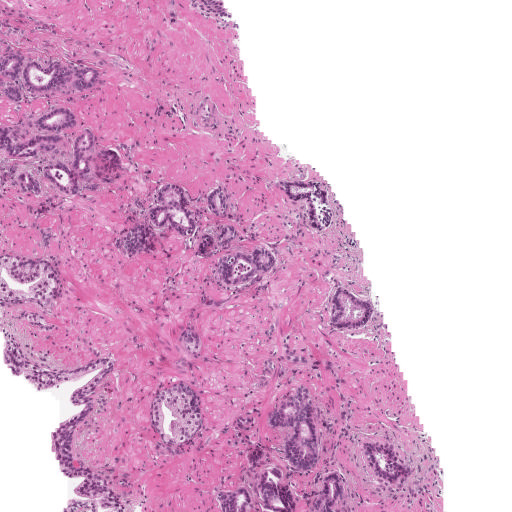
\includegraphics[width=0.35\linewidth]{stain_target_train.png}
\caption{\textbf{Training-derived Vahadane target.} The fixed target image used for training, validation, test, and WSI inference.}\end{figure}

\begin{figure}[H]\centering\includegraphics[width=\linewidth]{Fig05_augmentation.png}
\caption{\textbf{Training augmentations.} Seven configured transforms, each at its strongest setting, applied to one normalized L0 training patch.}\end{figure}

\subsection*{Patch-level audit}
The audit scores the stored test patches (at most two per class, level, and WSI). Overlapping patches count tissue locations repeatedly, and the L0 patches contribute 93.8\% of the audited pixels, so the pooled value is dominated by L0. These values are not comparable with the reconstructed WSI results.

\begin{table}[H]\centering\footnotesize
\caption{\textbf{Patch-level audit on the stored test patches.} Source: \texttt{paper\_results/tables/patch\_metrics\_per\_level\_and\_pooled.csv}.}
\begin{tabular}{lrrrrrr}\toprule
Subset & Dice & IoU & Precision & Recall & Specificity & Accuracy\\\midrule
L0 & 0.7799 & 0.6392 & 0.8333 & 0.7329 & 0.9614 & 0.9138\\
L1 & 0.8309 & 0.7107 & 0.8491 & 0.8135 & 0.9620 & 0.9310\\
L2 & 0.8037 & 0.6718 & 0.7995 & 0.8079 & 0.9323 & 0.9011\\
all levels pooled & 0.7831 & 0.6436 & 0.8343 & 0.7379 & 0.9614 & 0.9148\\
\bottomrule\end{tabular}\end{table}

\begin{figure}[H]\centering\includegraphics[width=\linewidth]{Fig10_confusion.png}
\caption{\textbf{Patch-level confusion matrices.} (A) Pooled across levels, (B) L0, (C) L1, and (D) L2.}\end{figure}

\subsection*{Supporting analyses}
\begin{table}[H]\centering\footnotesize
\caption{\textbf{Paired comparisons of fusion and single levels within each provider (common scoring region, 10,000 WSI resamples).} Source: \texttt{revision\_2026-10-30/tables/A1\_provider\_paired\_contrasts.csv}.}
\begin{tabular}{lllrrll}\toprule
Provider & Estimand & Contrast & WSI $n$ & Difference & 95\% CI & Holm $p$\\\midrule
Karolinska & pooled & Fusion$-$L0 & 818 & 0.1016 & [0.0929, 0.1110] & $<$0.0006\\
Karolinska & pooled & Fusion$-$L1 & 818 & $-$0.0002 & [$-$0.0059, 0.0057] & 0.9570\\
Karolinska & pooled & Fusion$-$L2 & 818 & 0.0379 & [0.0295, 0.0470] & $<$0.0006\\
Karolinska & per slide & Fusion$-$L0 & 526 & 0.0904 & [0.0776, 0.1032] & $<$0.0006\\
Karolinska & per slide & Fusion$-$L1 & 526 & $-$0.0317 & [$-$0.0429, $-$0.0208] & $<$0.0006\\
Karolinska & per slide & Fusion$-$L2 & 526 & 0.0987 & [0.0804, 0.1180] & $<$0.0006\\
Radboud & pooled & Fusion$-$L0 & 759 & 0.0503 & [0.0420, 0.0592] & $<$0.0006\\
Radboud & pooled & Fusion$-$L1 & 759 & 0.0323 & [0.0271, 0.0382] & $<$0.0006\\
Radboud & pooled & Fusion$-$L2 & 759 & 0.2078 & [0.1988, 0.2175] & $<$0.0006\\
Radboud & per slide & Fusion$-$L0 & 600 & 0.0492 & [0.0379, 0.0608] & $<$0.0006\\
Radboud & per slide & Fusion$-$L1 & 600 & 0.0239 & [0.0176, 0.0307] & $<$0.0006\\
Radboud & per slide & Fusion$-$L2 & 600 & 0.2497 & [0.2365, 0.2635] & $<$0.0006\\
\bottomrule\end{tabular}\end{table}

\begin{table}[H]\centering\footnotesize
\caption{\textbf{Design-effect sensitivity of the fusion-minus-L1 contrasts (common scoring region). The variance is inflated by $1+(m-1)\rho$ with $m$ the expected number of test WSIs per patient.} Source: \texttt{revision\_2026-10-30/tables/B2\_design\_effect.csv}.}
\begin{tabular}{lrrrlr}\toprule
Estimand & Difference & $\rho$ & Design effect & Inflated 95\% CI & Design effect for CI to reach 0\\\midrule
pooled & 0.0106 & 0.25 & 1.15 & [0.0059, 0.0153] & 5.78\\
pooled & 0.0106 & 0.50 & 1.30 & [0.0056, 0.0156] & 5.78\\
pooled & 0.0106 & 1.00 & 1.60 & [0.0050, 0.0162] & 5.78\\
per slide & $-$0.0021 & 0.25 & 1.15 & [$-$0.0090, 0.0049] & 0.10\\
per slide & $-$0.0021 & 0.50 & 1.30 & [$-$0.0094, 0.0053] & 0.10\\
per slide & $-$0.0021 & 1.00 & 1.60 & [$-$0.0102, 0.0061] & 0.10\\
\bottomrule\end{tabular}\end{table}

\begin{table}[H]\centering\footnotesize
\caption{\textbf{Detection of reference tumor components (8-connected on the evaluation grid) by size. A component counts as detected when the map predicts tumor on any of its pixels (common scoring region). On Radboud WSIs, components are mostly single glands, not lesions.} Source: \texttt{revision\_2026-10-30/tables/B6\_foci\_detection.csv}.}
\begin{tabular}{llrrr}\toprule
Provider & Area (mm$^2$) & Components & Detected by fusion (\%) & Detected by L1 (\%)\\\midrule
Karolinska & <0.01 & 146 & 67.8 & 60.3\\
Karolinska & 0.01-0.05 & 41 & 63.4 & 56.1\\
Karolinska & 0.05-0.25 & 149 & 79.2 & 81.9\\
Karolinska & 0.25-1 & 444 & 95.5 & 95.3\\
Karolinska & >=1 & 474 & 99.8 & 99.6\\
Pooled & <0.01 & 155,379 & 66.8 & 70.8\\
Pooled & 0.01-0.05 & 8,646 & 98.1 & 96.2\\
Pooled & 0.05-0.25 & 1,970 & 98.0 & 96.3\\
Pooled & 0.25-1 & 694 & 97.1 & 96.7\\
Pooled & >=1 & 490 & 99.8 & 99.6\\
Radboud & <0.01 & 155,233 & 66.8 & 70.8\\
Radboud & 0.01-0.05 & 8,605 & 98.2 & 96.4\\
Radboud & 0.05-0.25 & 1,821 & 99.6 & 97.5\\
Radboud & 0.25-1 & 250 & 100.0 & 99.2\\
Radboud & >=1 & 16 & 100.0 & 100.0\\
\bottomrule\end{tabular}\end{table}

\begin{table}[H]\centering\footnotesize
\caption{\textbf{Tumor-bearing test WSIs without any true-positive fused pixel.} Source: \texttt{revision\_2026-10-30/tables/B6\_complete\_misses.csv}.}
\begin{tabular}{lrrlrrr}\toprule
Provider & Reference tumor (mm$^2$) & Components & Empty prediction & L0 TP & L1 TP & L2 TP\\\midrule
Radboud & 0.0001 & 1 & no & 2 & 0 & 0\\
Radboud & 0.0002 & 1 & no & 0 & 0 & 0\\
Radboud & 0.0002 & 1 & yes & 0 & 0 & 0\\
Radboud & 0.0079 & 4 & yes & 93 & 0 & 0\\
Radboud & 0.0251 & 2 & no & 304 & 0 & 0\\
Radboud & 0.0264 & 12 & no & 9 & 0 & 0\\
Karolinska & 0.0296 & 1 & yes & 118 & 0 & 0\\
Radboud & 0.0543 & 2 & yes & 348 & 0 & 0\\
Radboud & 0.1231 & 32 & yes & 58 & 0 & 0\\
Radboud & 0.2178 & 23 & no & 1837 & 81 & 0\\
Karolinska & 0.2445 & 1 & yes & 2044 & 0 & 0\\
Karolinska & 0.3767 & 1 & yes & 1974 & 0 & 0\\
Karolinska & 0.3900 & 1 & no & 932 & 0 & 0\\
Karolinska & 0.4136 & 1 & no & 29 & 0 & 0\\
Karolinska & 0.5331 & 1 & yes & 1334 & 0 & 0\\
Karolinska & 0.6944 & 1 & no & 3675 & 0 & 0\\
Karolinska & 2.0434 & 1 & yes & 13028 & 0 & 0\\
\bottomrule\end{tabular}\end{table}

\begin{table}[H]\centering\footnotesize
\caption{\textbf{Reference-negative test WSIs by PANDA slide-level ISUP grade.} Source: \texttt{revision\_2026-10-30/tables/D3\_negative\_slides\_by\_grade.csv}.}
\begin{tabular}{llrrr}\toprule
Provider & Slide-level grade & WSIs & With false positives & Median false-positive area (mm$^2$)\\\midrule
Karolinska & ISUP 0 (benign) & 289 & 119 & 0.0000\\
Karolinska & ISUP >= 1 & 3 & 1 & 0.0000\\
Radboud & ISUP 0 (benign) & 143 & 104 & 0.0198\\
Radboud & ISUP >= 1 & 16 & 10 & 0.0037\\
\bottomrule\end{tabular}\end{table}

\begin{table}[H]\centering\footnotesize
\caption{\textbf{Boundary metrics of the fused map with the implementation's empty-boundary convention (all defined WSIs).} Source: \texttt{paper\_results/tables/boundary\_metrics\_summary.csv}.}
\begin{tabular}{lrrrrrrr}\toprule
metric & n defined & n undefined & mean & median & sd & min & max\\\midrule
fusion hd95 eval px & 1334 & 243 & 77.45 & 10.1 & 189.1 & 0 & 1863\\
fusion assd eval px & 1334 & 243 & 16.91 & 2.393 & 49.53 & 0 & 605.6\\
fusion surface dice & 1577 & 0 & 0.6626 & 0.8349 & 0.3645 & 0 & 1\\
fusion hd95 level0 px & 1334 & 243 & 1239 & 161.6 & 3025 & 0 & 2.98e+04\\
fusion assd level0 px & 1334 & 243 & 270.6 & 38.3 & 792.5 & 0 & 9690\\
\bottomrule\end{tabular}\end{table}

\begin{table}[H]\centering\footnotesize
\caption{\textbf{First SICAPv2 run on 18,765 patches of a renamed Kaggle copy (all patches of its Train folder; constant coordinate). Replaced in the main text by the evaluation of the official release.} Source: \texttt{external\_sicapv2/results/tables/global\_external\_metrics.json}.}
\begin{tabular}{lr}\toprule
Metric & Value\\\midrule
dice & 0.5737\\
iou & 0.4022\\
precision & 0.4928\\
recall & 0.6864\\
specificity & 0.7926\\
accuracy & 0.7685\\
\bottomrule\end{tabular}\end{table}

\begin{table}[H]\centering\footnotesize
\caption{\textbf{SICAPv2 official release: all patch sets, per patch and deduplicated, with constant and region-derived coordinates.} Source: \texttt{external\_sicapv2\_official/summary/SICAP\_official\_summary.csv}.}
\begin{tabular}{lllrrr}\toprule
Patch set & Scored unit & Coordinates & Dice & Precision & Recall\\\midrule
test partition & patch & constant & 0.6535 & 0.5844 & 0.7412\\
test partition & patch & region-derived & 0.6548 & 0.5911 & 0.7338\\
test partition & deduplicated pixel & constant & 0.6277 & 0.5346 & 0.7601\\
test partition & deduplicated pixel & region-derived & 0.6290 & 0.5405 & 0.7520\\
partition listed & patch & constant & 0.6525 & 0.6162 & 0.6932\\
partition listed & patch & region-derived & 0.6524 & 0.6212 & 0.6869\\
partition listed & deduplicated pixel & constant & 0.6447 & 0.5882 & 0.7130\\
partition listed & deduplicated pixel & region-derived & 0.6442 & 0.5933 & 0.7047\\
unlisted & patch & constant & 0.0023 & 0.0012 & 0.4701\\
unlisted & patch & region-derived & 0.0023 & 0.0012 & 0.4602\\
all & patch & constant & 0.5713 & 0.4859 & 0.6931\\
all & patch & region-derived & 0.5726 & 0.4909 & 0.6868\\
all & deduplicated pixel & constant & 0.5882 & 0.4992 & 0.7160\\
all & deduplicated pixel & region-derived & 0.5889 & 0.5042 & 0.7077\\
\bottomrule\end{tabular}\end{table}

\end{document}
